\subsection{U-Boot Falcon Mode}

\begin{frame}{Goal: boot faster!}
  \begin{columns}
  \column{0.4\textwidth}
  U-Boot Falcon Mode is about reducing the time spent in the bootloader.
  \column{0.6\textwidth}
  \begin{center}
  \vspace{1cm}
  
\includegraphics[height=0.6\textheight]{slides/boot-time-u-boot-falcon-mode/2falcons.pdf}\\
  \small Falcons are the fastest animals on Earth!\\
  \tiny Image credits:
  \url{https://openclipart.org/detail/287044/falcon-2}
  \end{center}
  \end{columns}
\end{frame}

\begin{frame}{Example: booting on Microchip SAMA5D36}
  \small You first need to understand how your SoC boots:
  \begin{columns}
    \column{0.5\textwidth}
    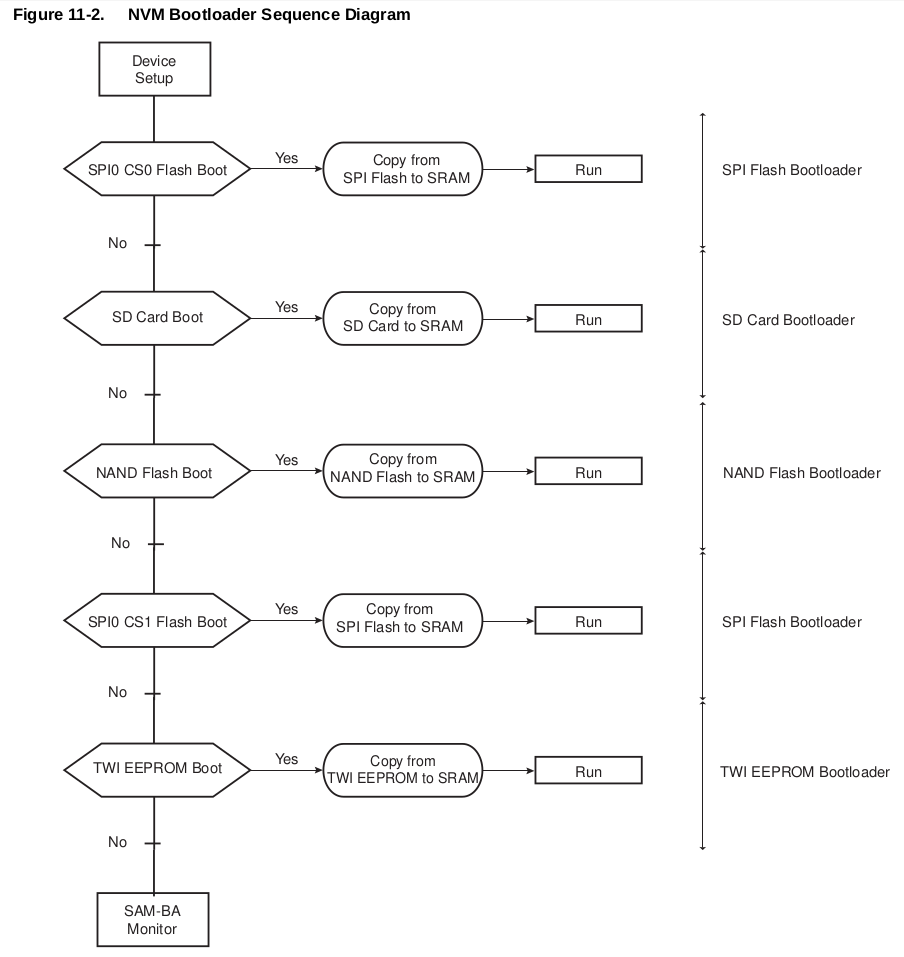
\includegraphics[height=0.7\textheight]{slides/boot-time-u-boot-falcon-mode/sama5d36-boot-diagram.png}
    \column{0.5\textwidth}
    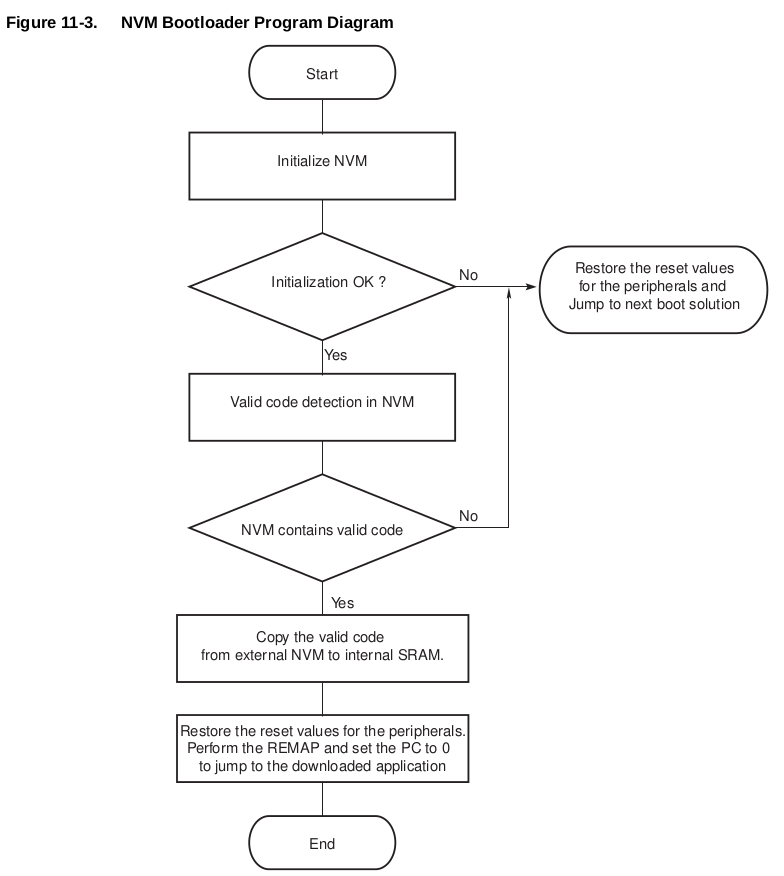
\includegraphics[height=0.7\textheight]{slides/boot-time-u-boot-falcon-mode/sama5d36-nvm-bootloader-program.png}
  \end{columns}
  \tiny Source: Microchip SAMA5D36 datasheet\\
  \url{https://ww1.microchip.com/downloads/en/DeviceDoc/Atmel-11121-32-bit-Cortex-A5-Microcontroller-SAMA5D3_Datasheet_B.pdf}
\end{frame}

\begin{frame}
  \frametitle{Normal and Falcon boot on Microchip SAMA5D3}
  \begin{columns}
    \column{0.2\textwidth}
    \begin{center}
    \includegraphics[width=\textwidth]{slides/boot-time-u-boot-falcon-mode/at91-boot.pdf}\\
    \vspace{0.5cm}
    \tiny Boot process with U-Boot
    \end{center}
    \column{0.7\textwidth}
    \footnotesize
    \begin{itemize}
    \item {\bf RomBoot}: tries to find a valid bootstrap image from
      various storage sources, and load it into SRAM (DRAM not
      initialized yet). Size limited to the SRAM size (here 64 KB).
    \item {\bf U-Boot SPL} ({\em Secondary Program Loader}):
       runs from SRAM (inside the SoC). Initializes the DRAM
       controller plus storage devices (MMC, NAND), loads the
       secondary bootloader into DRAM and starts it. Much bigger
       size limits!
    \item {\bf U-Boot}: runs from DRAM. Initializes other hardware
      devices (network, USB, etc.). Loads the kernel image from
      storage or network to DRAM and starts it.\\
      {\em This is the part that can be skipped}
    \item {\bf Linux Kernel}: runs from DRAM. Takes over the system
      completely (the bootloader no longer exists).
    \end{itemize}
    This scheme applies to all modern SoCs.
    \column{0.2\textwidth}
    \vspace{1cm}
    \begin{center}
    \includegraphics[width=\textwidth]{slides/boot-time-u-boot-falcon-mode/at91-falcon-boot.pdf}\\
    \vspace{0.5cm}
    \tiny Boot process without U-Boot ({\em Falcon mode})
    \end{center}
  \end{columns}
\end{frame}

\begin{frame}{Falcon mode advantages and drawbacks}
  \begin{itemize}
     \item Main advantage: since Linux and U-Boot are both loaded to RAM,\\
           U-Boot's {\em Falcon Mode} mainly saves time by directly loading Linux from the SPL
           instead of loading and executing the full U-Boot first.
     \item Drawback: you lose the flexibility brought by the full
           U-Boot. You have to follow a special procedure to update the kernel
           binary, DTB and kernel command line parameters.
     \item Advantage: the interactivity offered by the full U-Boot is
           not necessary on a production device. Falcon boot works in
           the same way on all SoCs on which U-Boot SPL is supported.
	   This makes it easier to apply this technique on all your
	   projects!
  \end{itemize}
\end{frame}

\begin{frame}{What U-Boot does (1)}
  U-Boot has multiple ways of preparing the kernel boot:
  \begin{itemize}
    \item {\em ATAGS} - The old way (before Device Tree)\\
          U-Boot prepares the Linux kernel command
	  line (\code{bootargs}), the machine ID and other information for Linux in
	  a tagged list, and passes its address to Linux through a
	  register.
    \item {\em Flattened Device Tree} - The standard way
    \begin{itemize}
	\item U-Boot checks the device tree loaded in RAM
	      or directly provides its own.
	\item U-Boot checks the specifics of the hardware
	      (amount and location of RAM, MAC address, present
	      devices...), possibly loads corresponding Device Tree overlays,
	      and modifies (fixes-up) the Device Tree accordingly.
	\item U-Boot stores the Linux kernel command line
	      (\code{bootargs}) in the \code{chosen} section
	      in the Device Tree.
    \end{itemize}
  \end{itemize}
\end{frame}

\begin{frame}{What U-Boot does (2)}
  \begin{itemize}
    \item {\em FIT Image} - The new way
    \begin{itemize}
	\item U-Boot loads the kernel(s), device tree(s), initramfs
	      image(s), signature(s) from a single file ({\em FIT Image})
	\item That's used for secure booting, for booting recovery
	      images, etc.
	\item U-Boot also implements Device Tree fix-ups, of course.
    \end{itemize}
  \end{itemize}
  Using the \code{spl export} command in U-Boot, you can do such
  preparation work ahead of time.

  \begin{itemize}
     \item In this presentation, we just cover standard Device Tree
	   booting.
     \item U-Boot also has support for FIT Image loading in the SPL, but
           that may still be a bit experimental, and such code must fit
           within your maximum allowable size for the SPL.\\
           See \projfile{u-boot}{arch/arm/cpu/armv8/fsl-layerscape/doc/README.falcon}
  \end{itemize}
\end{frame}

\begin{frame}{Falcon mode usage overview (1)}
   Here are the generic steps you need to go through:
   \begin{itemize}
     \item Recompile U-Boot with support for Falcon Mode
           (\projconfig{u-boot}{CONFIG_SPL_OS_BOOT}), with support
	   for \code{spl export} (\projconfig{u-boot}{CONFIG_CMD_SPL}),
	   and for the way you want to boot.
     \item Also make sure that \projconfig{u-boot}{CONFIG_SPL_SIZE_LIMIT} is
	   set (find the SRAM size for your CPU, \code{0x10000} for
           SAMA5D36), otherwise, U-Boot won't complain when the SPL
	   is bigger.
     \item Build the kernel legacy \code{uImage} file from \code{zImage}
	   (see next slides)
     \item Set the kernel command line (\code{bootargs} environment variable)
     \item Load the \code{uImage}, initramfs (if any) and Device Tree images
	   to RAM as usual.
   \end{itemize}
\end{frame}

\begin{frame}{Falcon mode usage overview (2)}
   Continued...
   \begin{itemize}
     \item Have U-Boot execute the preprocessing before booting Linux,
           but stop right before doing it:\\
	   \code{spl export fdt <kernel-addr> <initramfs-addr> <dtb-addr>}
     \item Save the exported data ({\em ARGS}) from RAM to storage, in {\em Flattened Device
	   Tree} form, so that the SPL can load it and directly pass it to
           the Linux kernel. The below environment variables will help:
	   \begin{itemize}
		\item \code{fdtargsaddr}: location of {\em ARGS} in RAM
		\item \code{fdtargslen}: size of {\em ARGS} in RAM
	   \end{itemize}
     \item If supported by your board (code explanations given later),
	   set your \code{boot_os} environment variable to \code{yes/Yes/true/True/1}
           to enable direct OS booting.
   \end{itemize}
\end{frame}

\begin{frame}[fragile]
\frametitle{spl export example output}
  \begin{columns}
  \column{0.65\textwidth}
  \begin{block}{}
  \scriptsize
  \begin{verbatim}
=> fatload mmc 0:1 0x21000000 uImage
5483584 bytes read in 530 ms (9.9 MiB/s)
=> fatload mmc 0:1 0x22000000 dtb
27795 bytes read in 7 ms (3.8 MiB/s)
=> setenv bootargs console=ttyS0,115200
=> spl export fdt 0x21000000 - 0x22000000
## Booting kernel from Legacy Image at 21000000 ...
   Image Name:   Linux-5.12.6
   Image Type:   ARM Linux Kernel Image (uncompressed)
   Data Size:    5483520 Bytes = 5.2 MiB
   Load Address: 20008000
   Entry Point:  20008000
   Verifying Checksum ... OK
## Flattened Device Tree blob at 22000000
   Booting using the fdt blob at 0x22000000
   Loading Kernel Image
   Loading Device Tree to 2fb2c000, end 2fb35c92 ... OK
subcommand not supported
subcommand not supported
   Loading Device Tree to 2fb1f000, end 2fb2bc92 ... OK
Argument image is now in RAM: 0x2fb1f000
  \end{verbatim}
  \end{block}
  \column{0.35\textwidth}
    \begin{center}
    \vspace{0.5cm}
    
\includegraphics[height=0.6\textheight]{slides/boot-time-u-boot-falcon-mode/horus.pdf}\\
    \vspace{0.5cm}
    \tiny Image credits:\\
    \url{https://openclipart.org/detail/292953/horus}
    \end{center}
  \end{columns}
\end{frame}

\begin{frame}[fragile]
   \frametitle{How to create the uImage file}
   Microchip SAMA5D3 Xplained board example
   \begin{itemize}
      \item Need to know the loading address that should be used for
            your board. Usually on ARM32, it's the starting physical address of
	    RAM plus \code{0x8000}.
      \item Either generate it from the Linux build system:\\
	  \begin{block}{}
	  \begin{verbatim}
make LOADADDR=0x20008000 uImage
          \end{verbatim}
	  \end{block}
      \item Or generate it using U-Boot's \code{mkimage} command:\\
	  \begin{block}{}
	  \begin{verbatim}
mkimage -A arm -O linux -C none  -T kernel \
-a 0x20008000 -e 0x20008000 \
-n "Linux-5.12.6" \
-d arch/arm/boot/zImage arch/arm/boot/uImage
          \end{verbatim}
	  \end{block}
   \end{itemize}
\end{frame}

\begin{frame}[fragile]
\frametitle{U-Boot code changes to support a new board (1)}
\small
Your \code{board/<vendor>/<board>/<board>.c} file must at least\\
implement the \projfunc{u-boot}{spl_start_uboot} function.\\
Here's the most typical example:
\begin{block}{}
\begin{minted}[fontsize=\scriptsize]{c}
#ifdef CONFIG_SPL_OS_BOOT
int spl_start_uboot(void)
{
       if (CONFIG_IS_ENABLED(SPL_SERIAL_SUPPORT) && serial_tstc() && serial_getc() == 'c')
               /* break into full u-boot on 'c' */
               return 1;

       if (CONFIG_IS_ENABLED(SPL_ENV_SUPPORT)) {
               env_init();
               env_load();
               if (env_get_yesno("boot_os") != 1)
                       return 1;
       }
       return 0;
}
#endif
\end{minted}
\end{block}
\end{frame}

\begin{frame}[fragile]
\frametitle{U-Boot code changes to support a new board (2)}
If you cannot fit support for an environment in the SPL,\\
the \projfunc{u-boot}{spl_start_uboot} function can be simpler:
\begin{block}{}
\begin{minted}[fontsize=\scriptsize]{c}
#ifdef CONFIG_SPL_OS_BOOT
int spl_start_uboot(void)
{
       if (CONFIG_IS_ENABLED(SPL_SERIAL_SUPPORT) && serial_tstc() && serial_getc() == 'c')
               /* break into full u-boot on 'c' */
               return 1;

       return 0;
}
#endif
\end{minted}
\end{block}
\end{frame}

\begin{frame}[fragile]
\frametitle{U-Boot code changes to support a new board (3)}
Or even, if reading characters from the serial line doesn't work:
\begin{block}{}
\begin{minted}[fontsize=\small]{c}
#ifdef CONFIG_SPL_OS_BOOT
int spl_start_uboot(void)
{
       return 0;
}
#endif
\end{minted}
\end{block}
You may also need extra defines to be set, but you will find
which ones are missing at compile time.
\end{frame}

\begin{frame}[fragile]
\frametitle{How to fall back to U-Boot}
   \begin{columns}
   \column{0.7\textwidth}
   \begin{itemize}
     \item If supported by your board, hit the specified key on the
           serial console and back in U-Boot, disable the \code{boot_os}
	   environment variable. That's it.
     \item Otherwise, try to cause OS loading to fail. The easiest way
	   is to erase the kernel binary and if needed the \code{spl
	   export} output.
     \item If this doesn't work, re-compile and update the SPL without
	   Falcon mode support, or temporarily modify the
           \projfunc{u-boot}{spl_start_uboot} function
	   to always return \code{1}. This way, you don't lose your
	   configuration.
   \end{itemize}
   \column{0.3\textwidth}
      \begin{center}
      
\includegraphics[height=0.6\textheight]{slides/boot-time-u-boot-falcon-mode/falcon-blue.png}
      \end{center}
   \end{columns}
\end{frame}

\begin{frame}[fragile]
\frametitle{Booting from raw MMC - Proposed storage layout}
   \begin{columns}
    \column{0.5\textwidth}
	\small For use on Microchip SAMA5D3 Xplained\\
        \vspace{0.5cm}
	\scriptsize
	{\fontsize{7}{10}\selectfont
	\begin{tabular}{| l | c | c |}
	\hline
	\makecell{Offset\\ (512 b sector)} & \makecell{Offset\\ (bytes)} & Contents \\
	\hline
	0x0 & 0 & \makecell{MBR\\ (Master Boot Record)} \\
	0x100 & 128 KiB & SPL ARGS \\
	0x200 & 256 KiB & \code{u-boot.img} \\
	0x1000 & 2 MiB & uImage \\
	0x4000 & 16 MiB & Start of FAT partition \\
	\hline
	\end{tabular}
	}\\
    \column{0.5\textwidth}
	\begin{itemize}
	   \item A FAT partition is required to store the SPL file
	         (\code{boot.bin}). SAMA5D36 doesn't support an SPL file
		 on raw MMC (unlike i.MX6).
	   \item Caution: partition offsets should be a multiple of the {\em
		 segment} size, as indicated by the device's
	         \code{preferred_erase_size} attribute under
		 \code{/sys/bus/mmc/devices/}.
	\end{itemize}
   \end{columns}
\end{frame}

\begin{frame}[fragile]
\frametitle{Booting from raw MMC - Configuration}
	\small
	U-Boot configuration (starting from
        \code{sama5d3_xplained_mmc_defconfig}):\\
	\projconfigval{u-boot}{CONFIG_SPL_OS_BOOT}{y}\\
	\projconfigval{u-boot}{CONFIG_SPL_SIZE_LIMIT}{0x10000}\\
	\projconfigval{u-boot}{CONFIG_SPL_LEGACY_IMAGE_FORMAT}{y}\\
	\projconfigval{u-boot}{CONFIG_SPL_MMC}{y}\\
	\projconfigval{u-boot}{CONFIG_CMD_SPL}{y}\\
	\projconfigval{u-boot}{CONFIG_CMD_SPL_WRITE_SIZE}{0x7000}\\
	\projconfigval{u-boot}{CONFIG_SYS_MMCSD_RAW_MODE_U_BOOT_SECTOR}{0x200}\\
	\projconfignotset{u-boot}{CONFIG_SPL_FS_FAT}\\
        \begin{block}{include/configs/sama5d3\_xplained.h}
        \begin{minted}[fontsize=\tiny]{c}
#define CONFIG_SYS_MMCSD_RAW_MODE_ARGS_SECTOR 0x100  /* 256 KiB */
#define CONFIG_SYS_MMCSD_RAW_MODE_ARGS_SECTORS (CONFIG_CMD_SPL_WRITE_SIZE / 512)
#define CONFIG_SYS_MMCSD_RAW_MODE_KERNEL_SECTOR 0x1000 /* 2 MiB */
#define CONFIG_SYS_SPL_ARGS_ADDR 0x22000000
	\end{minted}
	\end{block}
\end{frame}

\begin{frame}[fragile]
\frametitle{Booting from Raw MMC - Writing to raw storage}
   \scriptsize
   \begin{columns}
    \column{0.5\textwidth}
    On your GNU/Linux host:
    \begin{itemize}
	\item Write U-Boot (using the same block size as sector size, to
	      get the same offsets):\\
	      \code{sudo dd if=u-boot.img of=/dev/sdc bs=512 seek=512 conv=sync}
	\item Write \code{uImage}:\\
	      \code{sudo dd if=uImage of=/dev/sdc bs=512 seek=4096 conv=sync}
	\item Reminder: in our case (SAMA5D36), the SPL is copied to
	      \code{boot.bin} in a FAT partition.
    \end{itemize}
    \column{0.5\textwidth}
    On your U-Boot target,\\
    after \code{spl export}:
    \begin{itemize}
	\item Select the right MMC\\
        device for \code{mmc write}:
	\begin{verbatim}
=> mmc list
Atmel mci: 0 (SD)
Atmel mci: 1

=> mmc dev 0
switch to partitions #0, OK
mmc0 is current device
\end{verbatim}
	\item Check the size of ARGS
\begin{verbatim}
=> printenv fdtargslen
\end{verbatim}

        \item Divide it by the sector size (512), and convert it to
              hexadecimal (round it up), and use the value to save the ARGS to raw MMC:
\begin{verbatim}
=> mmc write ${fdtargsaddr} 0x100 0x67
\end{verbatim}
	\item {\bf Caution}: the last argument of \code{mmc write} is a
	      {\bf number of sectors}. If you pass a number of bytes, you'll erase your
	      FAT partition!
    \end{itemize}
   \end{columns}
\end{frame}

\begin{frame}{Booting from Raw MMC - Results and notes}
  \scriptsize
  \begin{columns}
  \column{0.5\textwidth}
         Reference test
	\begin{itemize}
           \item Loading \code{zImage} and \code{dtb} from FAT through
                 \code{fatload} and using a zero \code{bootdelay}:\\
	         \code{setenv bootdelay 0}
	         \code{setenv bootcmd 'fatload mmc 0:1 0x21000000 zImage; fatload mmc 0:1 0x22000000; bootz 0x21000000 - 0x22000000'}
	   \item Not completely fair because we have the filesystem overhead, but that's the standard / easiest way on MMC.
		 We could have loaded images from raw MMC, but that's very inconvenient.
	   \item Best result (using \code{grabserial}):\\
		 \code{[3.452681 0.000099] Please press Enter to activate this console.}
	\end{itemize}
  \column{0.5\textwidth}
        Falcon boot test
	\begin{itemize}
	   \item Best result:\\
		 \code{[3.191228 0.000134] Please press Enter to activate this console.}
	   \item We saved 261 ms, but that's disappointing.
	   \item Adding instrumentation to the SPL allowed us to understand why:
	   \begin{itemize}
	      \scriptsize
	      \item Time to load the kernel from U-Boot / FAT: 530 ms
	      \item Time to load the kernel from SPL / raw MMC: 1.010 ms
	   \end{itemize}
	   \item Here the specific MMC driver in SPL has poor performance (lack
		 of DMA?)
           \item We had much better results on different hardware, such
	         as saving 1.2s on i.MX6, and 1.05s on TI AM3358
                 (Beagle Bone Black, loading from FAT with U-Boot SPL
                 2022.04).
	\end{itemize}
  \end{columns}
\end{frame}

\begin{frame}[fragile]
\frametitle{Booting from raw NAND - Configuration}
   \begin{columns}
    \column{0.5\textwidth}
	\footnotesize
	Proposed NAND layout\\
        For use on Microchip SAMA5D3 Xplained\\
        \vspace{0.5cm}
	{\fontsize{7}{10}\selectfont
	\begin{tabular}{| l | c | c |}
	\hline
	Offset & Size & Contents \\
	\hline
	0x0 & 256 KiB & SPL (\code{spl/u-boot-spl.bin})\\
	0x40000 & 1 MiB & U-Boot (\code{u-boot.bin}) \\
	0x140000 & 128 KiB & U-Boot redundant environment \\
	0x160000 & 128 KiB & U-Boot environment \\
	0x180000 & 128 KiB & Original DTB or CMD \\
	0x1a0000 & 6.375 MiB & uImage \\
	0x800000 & & Other partitions \\
	\hline
	\end{tabular}
	}\\
        \vspace{0.5cm}
	Notes:
	\begin{itemize}
	   \item Only the SPL offset is hardcoded
	   \item All others can be configured differently
	   \item Offsets must be a multiple of the erase block size (128 KiB)
	\end{itemize}
    \column{0.5\textwidth}
	\footnotesize
	U-Boot configuration\\
	\projconfigval{u-boot}{CONFIG_SPL_OS_BOOT}{y}
	\projconfigval{u-boot}{CONFIG_SPL_SIZE_LIMIT}{0x10000}
	\projconfigval{u-boot}{CONFIG_ENV_OFFSET}{0x160000}\\
	\projconfigval{u-boot}{CONFIG_ENV_OFFSET_REDUND}{0x140000}\\
	\projconfigval{u-boot}{CONFIG_SPL_LEGACY_IMAGE_FORMAT}{y}\\
	\projconfigval{u-boot}{CONFIG_SPL_NAND_SUPPORT}{y}\\
	\projconfigval{u-boot}{CONFIG_SPL_NAND_DRIVERS}{y}\\
	\projconfigval{u-boot}{CONFIG_SPL_NAND_BASE}{y}\\
	\projconfigval{u-boot}{CONFIG_CMD_SPL_WRITE_SIZE}{0x7000}\\
	\projconfigval{u-boot}{CONFIG_CMD_SPL_NAND_OFS}{0x180000}\\
        (starting from
        \code{sama5d3_xplained_nandflash_defconfig})

        \begin{block}{include/configs/sama5d3\_xplained.h}
        \begin{minted}[fontsize=\tiny]{c}
/* Generic settings */
#define CONFIG_SYS_NAND_U_BOOT_OFFS     0x40000

/* Falcon boot support on raw NAND */
#define CONFIG_SYS_NAND_SPL_KERNEL_OFFS 0x1a0000
	\end{minted}
	\end{block}
   \end{columns}
\end{frame}

\begin{frame}{Booting from raw NAND - Results and notes}
  \small
  \begin{itemize}
     \item Reference test
	\begin{itemize}
           \item To be fair, using a zero \code{bootdelay} and the exact \code{zImage} and \code{dtb} size:\\
	         \code{setenv bootdelay 0}
	         \code{setenv bootcmd 'nand read 0x21000000 0x1a0000 0x53ac00; nand read 0x22000000 0x180000 0x6c93; bootz 0x21000000 - 0x22000000'}
	   \item Best result (using \code{grabserial}):\\
		 \code{[4.320618 0.000470] Please press Enter to activate this console.}
	\end{itemize}
     \item Falcon boot test
	\begin{itemize}
	   \item Best result (using \code{grabserial}):\\
		 \code{[3.768543 0.000125] Please press Enter to activate this console.}
	   \item We saved 552 ms!
	\end{itemize}
  \end{itemize}
\end{frame}

\begin{frame}{U-Boot code and debugging Falcon Mode}
  \begin{columns}
  \column{0.7\textwidth}
  \begin{itemize}
     \item Depending on how you boot, read the corresponding code:
        \begin{itemize}
	   \item \projfile{u-boot}{common/spl/spl_mmc.c}
	   \item \projfile{u-boot}{common/spl/spl_nand.c}
	   \item Other files in \projfile{u-boot}{common/spl/}
	\end{itemize}
     \item If booting doesn't work, the easiest way is to add
	   \code{puts();} lines to trace strategic functions
	   and check return values. You'll get the messages in the
	   serial console.
  \end{itemize}
  \column{0.3\textwidth}
    \begin{center}
     
\includegraphics[height=0.6\textheight]{slides/boot-time-u-boot-falcon-mode/falcon-red.png}
    \end{center}
  \end{columns}
\end{frame}

\begin{frame}{Issues and lessons learned (1)}
   \begin{itemize}
      \item {\em SPL storage driver performance}: not on all platforms,\\
	    but at least here on Microchip SAMA5.
      \item {\em Features limited by space}: what can be done with
            Falcon booting is not limited by U-Boot features, but by how much code
	    can fit in the limited SRAM.\\
	    This is why I couldn't show Falcon booting from a FAT
            partition, because adding support for this filesystem and disk partitions to
	    the SPL doesn't fit in the maximum size possible on the particular
	    platform chosen for the demo.
      \item {\em U-Boot initializations}: in addition to the FDT fixups without which
            the Linux kernel may not boot, the Linux kernel may also rely on some
            initializations performed by U-Boot. Before such dependencies
	    can be removed by updating kernel drivers, you may need to
	    hardcode such initializations in the SPL, provided you have enough
	    space!
   \end{itemize}
\end{frame}

\begin{frame}{Issues and lessons learned (2)}
   \begin{itemize}
      \item {\em Limited automation}: while the \code{uImage} file can be updated
            automatically in the storage image, any change in the kernel
	    command line or Device Tree must go through the \code{spl export} command
            {\bf on the board}. The FDT fixups done by U-Boot are not trivial to
            reproduce. This makes it difficult to prepare production images without a
            manual step in U-Boot.
      \item {\em No decompression}: U-Boot currently doesn't seem to
	    support decompression in the SPL. If your architecture
            doesn't support kernel self-decompression and relies on the bootloader
	    (e.g. arm64 or riscv), Falcon mode won't be available if you are using
	    a compressed kernel.
      \item Falcon mode severely complicates the implementation of A/B updates,
	    as all the logic to switch between versions should be implemented
	    in the SPL.
      \item {\em Side note}: Found that U-Boot's \code{bootm} was
	    noticeably slower than \code{bootz} (+170 ms)
   \end{itemize}
\end{frame}

\begin{frame}{Further work}
   \begin{columns}
   \column{0.7\textwidth}
   \begin{itemize}
      \item Improve raw MMC read performance in the SPL on Microchip SAMA5
      \item Didn't try with what U-Boot calls the {\em Raw} kernel
            images yet, supported with \projconfig{u-boot}{CONFIG_SPL_RAW_IMAGE_SUPPORT}.
            Assuming this corresponds to the \code{arch/arm/boot/Image}
      \item Didn't try FIT Image support in SPL yet. Will try on an SoC
	    with more space for SPL (i.MX)
   \end{itemize}
   \column{0.3\textwidth}
    \begin{center}
     \vspace{1cm}
     
\includegraphics[width=\textwidth]{slides/boot-time-u-boot-falcon-mode/millenium-falcon.pdf}\\
     \vspace{1cm}
     \tiny Image credits:\\
     \url{https://openclipart.org/detail/224913/clip-is-a-brick-star-wars-millenium-falcon-set-4488}
    \end{center}
   \end{columns}
\end{frame}

\begin{frame}{References}
   \begin{itemize}
      \item Bootlin's commit to support Falcon boot on SAMA5D3 Xplained in mainline U-Boot:
	    {\small \url{https://source.denx.de/u-boot/u-boot/-/commit/ea83ea5afd18}}
      \item U-Boot's \projfile{u-boot}{doc/README.falcon} file
      \item Linus Walleij: {\em How the ARM32 kernel decompresses}:\\
	    \small\url{https://people.kernel.org/linusw/how-the-arm32-linux-kernel-decompresses}
   \end{itemize}
\end{frame}

\setuplabframe
{Reduce bootloader time}
{
\begin{itemize}
\item Experiment with faster storage
\item Skipping U-Boot through the {\em Falcon Mode}, directly booting
      Linux from U-Boot SPL.
\item Measuring the final boot time.
\end{itemize}
}

